%%
%% Copyright 2007-2019 Elsevier Ltd
%%
%% This file is part of the 'Elsarticle Bundle'.
%% ---------------------------------------------
%%
%% It may be distributed under the conditions of the LaTeX Project Public
%% License, either version 1.2 of this license or (at your option) any
%% later version.  The latest version of this license is in
%%    http://www.latex-project.org/lppl.txt
%% and version 1.2 or later is part of all distributions of LaTeX
%% version 1999/12/01 or later.
%%
%% The list of all files belonging to the 'Elsarticle Bundle' is
%% given in the file `manifest.txt'.
%%

%% Template article for Elsevier's document class `elsarticle'
%% with numbered style bibliographic references
%% SP 2008/03/01
%%
%%
%%
%% $Id: elsarticle-template-num.tex 168 2019-02-25 07:15:41Z apu.v $
%%
%%
\documentclass[preprint,review,12pt]{elsarticle}


%% Use the option review to obtain double line spacing
% \documentclass[authoryear,preprint,review,12pt]{elsarticle}

%% Use the options 1p,twocolumn; 3p; 3p,twocolumn; 5p; or 5p,twocolumn
%% for a journal layout:
%% \documentclass[final,1p,times]{elsarticle}
%% \documentclass[final,1p,times,twocolumn]{elsarticle}
%% \documentclass[final,3p,times]{elsarticle}
% \documentclass[final,3p,times,twocolumn]{elsarticle}
%% \documentclass[final,5p,times]{elsarticle}
%% \documentclass[final,5p,times,twocolumn]{elsarticle}

%% For including figures, graphicx.sty has been loaded in
%% elsarticle.cls. If you prefer to use the old commands
%% please give \usepackage{epsfig}

%% The amssymb package provides various useful mathematical symbols
\usepackage{amssymb}
%% The amsthm package provides extended theorem environments
% \usepackage{amsthm}

%% The lineno packages adds line numbers. Start line numbering with
%% \begin{linenumbers}, end it with \end{linenumbers}. Or switch it on
%% for the whole article with \linenumbers.
%% \usepackage{lineno}

%%!!!!user's commands
\usepackage{amsmath}
\newcommand{\angstrom}{\text{\normalfont\AA}}

\newcommand{\hmn}[1]{% Hermann-Maguin notation
  \ensuremath{\begingroup\setupHMN #1\endgroup}%
}

\newcommand{\setupHMN}{%
  \doHMN{-}{\HMNoverline}%
  \doHMN{*}{\HMNminverse}%
  \doHMN{i}{\infty}
}

\newcommand{\doHMN}[2]{%
  \begingroup\lccode`~=`#1
  \lowercase{\endgroup\let~}#2%
  \mathcode`#1="8000
}

\newcommand{\HMNminverse}[1]{\frac{#1}{m}}
\newcommand{\HMNoverline}[1]{\mkern1mu\overline{\mkern-1mu#1\mkern-1mu}\mkern1mu}

\usepackage{miller}
\usepackage{multirow}
\usepackage{xcolor}
\usepackage{subfigure}
\usepackage[breaklinks]{hyperref}
\usepackage{graphicx}

\journal{Journal of Solid State Chemistry}

\begin{document}

\begin{frontmatter}

%% Title, authors and addresses

%% use the tnoteref command within \title for footnotes;
%% use the tnotetext command for theassociated footnote;
%% use the fnref command within \author or \address for footnotes;
%% use the fntext command for theassociated footnote;
%% use the corref command within \author for corresponding author footnotes;
%% use the cortext command for theassociated footnote;
%% use the ead command for the email address,
%% and the form \ead[url] for the home page:
%% \title{Title\tnoteref{label1}}
%% \tnotetext[label1]{}
%% \author{Name\corref{cor1}\fnref{label2}}
%% \ead{email address}
%% \ead[url]{home page}
%% \fntext[label2]{}
%% \cortext[cor1]{}
%% \address{Address\fnref{label3}}
%% \fntext[label3]{}

\title{Supplementary Material \--- Laves polyhedra in synthetic tennantite, Cu\textsubscript{12}As\textsubscript{4}S\textsubscript{13}, and its lattice dynamics}

\author[TISNCM]{Alexey~A.~Yaroslavzev}
\ead{yaroslavzevalex@gmail.com}
\author[MSU,ICRAS]{Alexey~N.~Kuznetsov}
\author[SIC]{Alexander~P.~Dudka}
\author[MSU]{Andrei~V.~Mironov}
\author[MIPT,TISNCM]{Sergey~G.~Buga}
\author[TISNCM]{Vladimir~V.~Denisov}

\address[TISNCM]{Technological Institute for Superhard and Novel Carbon Materials, 108840, Troitsk, Moscow, Russia}
\address[MSU]{Department of Chemistry, Lomonosov Moscow State University, 119991, Moscow, Russia}
\address[ICRAS]{Kurnakov Institute of General and Inorganic Chemistry RAS, 119991, Moscow, Russia}
\address[SIC]{Shubnikov Institute of Crystallography of Federal Scientific Research Centre “Crystallography and Photonics” of Russian Academy of Sciences, Leninskiy Prospekt 59, 119333, Moscow, Russia}
\address[MIPT]{Moscow Institute of Physics and Technology, 141700, 9 Institutsky lane, Dolgoprudny, Russia}


\end{frontmatter}


\section{A spherical shape single-crystal X-ray diffraction study}\label{sec:level1}

A~spherical shape single-crystal sample of Cu\textsubscript{12}As\textsubscript{4}S\textsubscript{13}  was prepared for the anisotropic extinction study.
Table~\ref{tab:inter_dist} and in~Table~\ref{tab:crystallographic_information} show the~comparison of previous results\cite{yaroslavzev2019} and the spherical shape single-crystal structural data. Refined atomic parameters and refined anisotropic ADP are presented in~Table~\ref{tab:atom_param} and in~Table~\ref{tab:ref_adp}.

\begin{table}
\caption{\label{tab:inter_dist}
Interatomic distances in Cu\textsubscript{12}As\textsubscript{4}S\textsubscript{13}.}
\centering
\resizebox{\columnwidth}{!}{
\begin{tabular}{lccc}
Distance&
Averaged, \AA  &
Extinct, \AA  &
Ref.~\cite{yaroslavzev2019} at 293~K, \AA  \\
Cu1 -- S1$\times$4   & 2.3177(17) & 2.3147(10) & 2.3099(6) \\
Cu2 -- Cu21$\times$2 & 0.890(17)  & 0.868(9)   & 0.95(3) \\
Cu2 -- S1$\times$2   & 2.208(4)   & 2.211(3)   & 2.219(3) \\
Cu2 -- S2            & 2.219(6)   & 2.223(4)   & 2.206(5) \\
Cu21 -- S1$\times$2  & 2.421(18)  & 2.420(10)  & 2.427(17) \\
Cu21 -- S2           & 2.326(15)  & 2.316(10)  & 2.380(14) \\
As1 -- S1$\times$3   & 2.2543(19) & 2.2530(10) & 2.2457(19) \\
Cu21 -- As1          & 2.604(17)  & 2.626(10)  & 2.535(19) \\
Cu2 -- As1           & 3.4816(11) & 3.4813(7)  & 3.480(4) \\

\end{tabular}
}
\end{table}


\begin{table*} %The best place to locate the table environment is directly after its first reference in text
\caption{\label{tab:crystallographic_information}
Summary of crystallographic information for Cu\textsubscript{12}As\textsubscript{4}S\textsubscript{13} structural experiment.}
\centering
\resizebox{\textwidth}{!}{
\begin{tabular}{cccc}
&
Averaged &
Extiction&
Ref.~\cite{yaroslavzev2019}, 293~K \\

a, \AA                                                     & \multicolumn{2}{c}{10.1742(2)}	                              	             & 10.1572(2)	\\
V, \AA\textsuperscript{3}                                  & \multicolumn{2}{c}{1053.19(4)}	                              	             & 1047.91(4)	\\
S.G.                                                       & \multicolumn{3}{c}{ \hmn{I -4 3 m} }	                                             	\\
Radiation, wavelength (\AA)                                & \multicolumn{2}{c}{Ag K\textsubscript{$\alpha$}, 0.56089}		                & Mo K\textsubscript{$\alpha$}, 0.71069	\\
Diffractometer                                             & \multicolumn{2}{c}{CAD4}	                                                  & Xcalibur	\\
Absorption correction                                      & \multicolumn{2}{c}{Analytical (sphere)}	                    	             & Analytical (crystal shape)	\\
$\Theta$\textsubscript{max}, deg.                                 & \multicolumn{2}{c}{29.85}	                                  	             & 42.08	\\
R\textsubscript{int}                                       & 0.046	                                                     & ---	         & 0.049	\\
N\textsubscript{ref} , collected                           & \multicolumn{2}{c}{3509}	                                    	             & 11026	\\
N\textsubscript{ref} , independent, $I\geqslant2\sigma(I)$ & 570	                                                       & 2837	         & 667	\\
N\textsubscript{paf}                                       & 50	                                                         & 55	           & 44	\\
Refinement on                                              & \multicolumn{2}{c}{$|F|$}	                                	             & $|F|$	\\
Anharmonic, Atoms (rank)                                   & \multicolumn{2}{c}{Cu1(4), Cu2(3), Cu21(3), S1(3), As1(3)}	  	             & Cu1(4), Cu2(3), Cu21(3), S2(4)	\\
GOF                                                        & 1.01	                                                       & 1.04	         & 1.00	\\
R/{\it w}R\textsubscript{2}                                & 0.028/0.036	                                               & 0.038/0.050	 & 0.029/0.038	\\
Min. Negative JPDF, \% of positive                         & -2.7	                                                       & 	-3.8             & -3.4	\\
$\pm\Delta\rho$, {\it e}\AA\textsuperscript{-3}            & +0.64/–0.76	                                                 & +1.18/–0.61	 & +1.7/–1.2	\\


\end{tabular}}
\end{table*}

\begin{table}
\caption{\label{tab:atom_param}
Refined atomic parameters in Cu\textsubscript{12}As\textsubscript{4}S\textsubscript{13}. 
Cu(1): $\frac{1}{2}$,$\frac{1}{4}$,0; Cu(2): x,0,0; Cu(21): x,y,y; As(1): x,x,x;  S(1): x,y,–y; S(2): 0,0,0.}
\centering
\resizebox{\columnwidth}{!}{
\begin{tabular}{lccc}
&
Averaged, \AA  &
Extinct, \AA  &
Ref.~\cite{yaroslavzev2019} at 293~K, \AA  \\
Occupancy, Cu(2)                          & 0.660(8)    & 0.670(5)     & 0.679(11)  \\
x, Cu(2)                                  & 0.2181(6)   & 0.2185(4)    & 0.2172(5)  \\
x, Cu(21)                                 & 0.2113(15)  & 0.2111(10)   & 0.2149(12) \\
y, Cu(21)                                 & 0.0617(17)  & 0.0601(9)    & 0.0662(19) \\
x, As(1)                                  & 0.24141(10) & 0.24141(6)   & 0.24162(4) \\
x, S(1)                                   & 0.3566(2)   & 0.35709(12)  & 0.35722(7) \\
–y, S(1)                                  & 0.11809(14) & 0.11835(8)   & 0.11854(6) \\
Ueq$\times$10\textsuperscript{4}, Cu(1)   & 212(3)      & 214(2)       & 184(3)     \\
Ueq$\times$10\textsuperscript{4}, Cu(2)   & 399(8)      & 415(5)       & 339(5)     \\
Ueq$\times$10\textsuperscript{4}, Cu(21)  & 543(22)     & 573(13)      & 420(3)     \\
Ueq$\times$10\textsuperscript{4}, As(1)   & 146.8(5)    & 147.1(3)     & 114.0(7)   \\
Ueq$\times$10\textsuperscript{4}, S(1)    & 151.6(15)   & 152.5(10)    & 111.0(13)  \\
Ueq$\times$10\textsuperscript{4}, S(2)    & 164.6(14)   & 167.5(9)     & 160(7)     \\

\end{tabular}
}
\end{table}


\begin{table}
\caption{\label{tab:ref_adp}
Refined anisotropic ADP in Cu\textsubscript{12}As\textsubscript{4}S\textsubscript{13}.}
\centering
\resizebox{\columnwidth}{!}{
\begin{tabular}{lccc}
&
Averaged, \AA  &
Extinct, \AA  &
Ref.~\cite{yaroslavzev2019} at 293~K, \AA  \\
$U_{11}$, $U_{33}\times$10\textsuperscript{4}, Cu(1)             & 176(4)      & 179(3)     & 146(3)  \\
$U_{22}\times$10\textsuperscript{4}, Cu(1)                       & 284(9)      & 284(6)     & 248(7)  \\
$U_{11}\times$10\textsuperscript{4}, Cu(2)                       & 158(7)      & 148(9)     & 117(6)  \\
$U_{22}$, $U_{33}\times$10\textsuperscript{4}, Cu(2)             & 493(14)     & 537(14)    & 451(9)  \\
$U_{11}\times$10\textsuperscript{4}, Cu(21)                      & 210(20)     & 193(20)    & 205(18)  \\
$U_{22}$, $U_{33}\times$10\textsuperscript{4}, Cu(21)            & 660(70)     & 710(40)    & 490(60)  \\
$U_{12}$, $U_{13}\times$10\textsuperscript{4}, Cu(21)            & –140(40)    & –70(30)    & –170(30)  \\
$U_{23}\times$10\textsuperscript{4}, Cu(21)                      & 470(80)     & 530(50)    & 290(60)  \\
$U_{11}\times$10\textsuperscript{4}, S(1)                        & 134(4)      & 133(3)     & 90(3)  \\
$U_{22}$, $U_{33}\times$10\textsuperscript{4}, S(1)              & 163(2)      & 163.2(16)  & 119.9(18)  \\
$U_{12}$, $-U_{13}\times$10\textsuperscript{4}, S(1)             & –19.7(18)   & –22.0(14)  & –23.6(14)  \\
$U_{23}\times$10\textsuperscript{4}, S(1)                        & 2(3)        & 3(2)       & –8(2)  \\
$U_{11}$, $U_{22}$, $U_{33}\times$10\textsuperscript{4}, S(2)    & 166(4)      & 169(3)     & 128(3)  \\
$U_{11}$, $U_{22}$, $U_{33}\times$10\textsuperscript{4}, As(1)   & 151.9(15)   & 149.0(11)  & 112.8(13)  \\
$U_{12}$, $U_{13}$, $U_{23}\times$10\textsuperscript{4}, As(1)   & 1.4(12)     & 0.1(9)     & –1.6(10)  \\

\end{tabular}
}
\end{table}


\section{Data collection, Reduction and Model Refinement}\label{sec:level1}
A sample with the shape of an irregular parallelepiped with the sides of approximately 0.456~$\times$~0.312~$\times$~0.247~mm\textsuperscript{3} was used for the diffraction study. Five diffraction experiments were performed on Rigaku Oxford Diffraction's Xcalibur diffractometer with an EOS S2 CCD detector. Mo~K\textsubscript{$\alpha$} radiation with  $\lambda=0.71073$ \AA  wavelength was used. Measurements was made at nominal temperatures at
85, 115, 180, 250, and 293~K.
A~Cobra Plus cryosystem (Oxford Cryosystems) with an open stream of cold nitrogen directed at the specimen was used to cool.
In a process of low-temperature diffraction experiments, it was necessary to take into account a temperature gradient between the temperature sensor fixed in the nozzle of the cryostrimmer and the sample located at a distance of up to 12 mm from the sensor.
The calibration was performed\cite{Dudka2016_2}, and it shown that the actual sample temperatures were 90, 119, 182, 251, and 293~K. Data sets with a maximum reflex scattering angle of $\theta=42.0$, degrees and the data redundancy of more than 15.4 were obtained in experiments.

The calculation of integral intensities from diffraction patterns was performed using the CrysAlisPro program\cite{Rigaku}.
The data processing included: consideration of geometric features of the data collection (Lorentz correction) and correction for polarization of radiation; calibration of the diffractometer\cite{Dudka2010}; absorption correction for \textcolor{red}{polyhedra} samples (performed by the Gaussian integration method\cite{Busing1957}); refinement of the half-wavelength contribution\cite{Dudka2010_2}; the correction for an extinction\cite{Becker1974}.
The corrections and refinement of structural parameters were performed in the Jana2006\cite{Petek2014} and ASTRA programs\cite{Dudka2007}.
Fourier syntheses of the electron density were calculated using the Jana2006 program\cite{Petek2014}.
Graphic constructions were made in Diamond\cite{Diamont}, and Vesta programs\cite{Momma2011}.


\section{Atomic charge distribution}\label{sec:level1}

Table~\ref{tab:calc_energ} shows calculated Bader atomic charges.

\begin{table*}[t]
\caption{\label{tab:calc_energ}
Calculated Bader atomic charges in reference (0), and optimized (1-19) structures. Red marks As, and S1 charges in more covalent structures; blue marks As and S1 charges in intermediately ionic structures; bold marks the structures with an energy gain related to the reference; blue shading marks the structure with the lowest energy.
}
\centering
\resizebox{\textwidth}{!}{
\begin{tabular}{ccccccccccc}
Atom                  & 0   & 1   & 2   & 3   & 4   & 5   & 6   & 7   & 8   & 9 \\
Cu1                  & +0.57	                & +0.56	                  & {\bf +0.56 }	& {\bf +0.56 }	& +0.56	& +0.56	                  & +0.56	& +0.56	& +0.56	                  & {\bf +0.56} \\
\multirow{2}{*}{Cu2} & \multirow{2}{*}{+0.49}	& \multirow{2}{*}{+0.47}	& {\bf +0.45 }	& {\bf +0.49 }	& +0.47 & +0.51	                  & +0.49	& +0.49	& +0.49	                  & {\bf +0.50} \\
		                 &		                    &                         & {\bf +0.40 }	& {\bf +0.39 }	& +0.40	& +0.47	                  & +0.39	& +0.39	& +0.45	                  & {\bf +0.46} \\
\multirow{2}{*}{S1}  & -1.41	                & -1.45	                  & {\bf -1.42 }  & {\bf -1.42 }	& -1.39	& \textcolor{red}{-0.76}	& -1.43	& -1.43	& \textcolor{blue}{-0.73}	& \textcolor{blue}{-0.70} \\
                     & -1.47	                & -1.53	                  & {\bf -1.49 }  & {\bf -1.50 }	& -1.47	& \textcolor{red}{-0.92}	& -1.53	& -1.52	& \textcolor{blue}{-1.42}	& \textcolor{blue}{-1.44} \\
S2                   & -0.88	                & -0.85	                  & {\bf -0.78 }  & {\bf -0.82 }	& -0.84	& -0.84	                  & -0.83	& -0.83	& -0.86	                  & {\bf -0.86} \\
\multirow{2}{*}{As}  & \multirow{2}{*}{+2.97}	& +3.05	                  & {\bf +3.12 }	& {\bf +3.15 }	& +3.06	& +0.86	                  & +3.11	& +3.12	& \textcolor{blue}{+2.03}	& \textcolor{blue}{+1.51} \\
	                   &                        & +2.99	                  & {\bf +2.99 }  & {\bf +3.07 }	& +3.11	& +0.93	                  & +3.06	& +3.07	& \textcolor{blue}{+1.53}	& \textcolor{blue}{+0.89} \\

Atom                  & 10   & 11   & 12   & 13   & 14   & 15   & 16   & 17   & 18   & 19 \\
Cu1                  & +0.56   & 	{\bf +0.56 }           & 	+0.56  & 	+0.56                  & 	{\bf +0.56 }           & 	+0.56                  & 	+0.56                  & 	{\bf +0.56 }           & 	{\bf +0.56 }           & 	{\bf +0.56 } \\
\multirow{2}{*}{Cu2} & +0.48   & 	{\bf +0.51 }           & 	+0.46  & 	+0.51                  & 	{\bf +0.50 }           & 	+0.51                  & 	+0.51                  & 	{\bf +0.51 }           & 	{\bf +0.51 }           & 	{\bf +0.50 } \\
		                 & +0.39   & 	{\bf +0.48 }           & 	+0.45  & 	+0.47                  & 	{\bf +0.46 }           & 	+0.46                  & 	+0.45                  & {\bf +0.46 }            & 	{\bf +0.46 }           & 	{\bf +0.46 } \\
\multirow{2}{*}{S1}  & -1.43   & 	\textcolor{red}{-0.73} & 	-1.42  & 	\textcolor{red}{-0.72} & 	\textcolor{red}{-0.73} & 	\textcolor{red}{-0.73} & 	\textcolor{red}{-0.72} & 	\textcolor{red}{-0.72} & 	\textcolor{red}{-0.74} & 	\textcolor{red}{-0.72} \\
                     & -1.52   & 	\textcolor{red}{-0.76} & 	-1.52  & 	\textcolor{red}{-0.77} & 	\textcolor{red}{-0.76} & 	\textcolor{red}{-0.77} & 	\textcolor{red}{-0.77} & 	\textcolor{red}{-0.77} & 	\textcolor{red}{-0.76} & 	\textcolor{red}{-0.76} \\
S2                   & -0.82   & 	{\bf -0.98}            & 	-0.81  & 	-0.93                  & 	{\bf -0.90 }           & 	-0.94                  & 	-0.90                  & 	{\bf -0.88 }           & 	{\bf -0.91 }           & 	{\bf -0.89 } \\
\multirow{2}{*}{As}  & +3.11   & 	\textcolor{red}{+0.94} & 	+3.07  & \textcolor{red}{+0.94}  & 	\textcolor{red}{+0.94} & 	\textcolor{red}{+0.94} & 	\textcolor{red}{+0.95} & 	\textcolor{red}{+0.95} & 	\textcolor{red}{+0.91} & 	\textcolor{red}{+0.91} \\
	                   & +3.00	 & \textcolor{red}{+0.76}	 & +2.99	 & \textcolor{red}{+0.85}	 & \textcolor{red}{+0.80}	 & \textcolor{red}{+0.84}	 & \textcolor{red}{+0.87}	 & \textcolor{red}{+0.85}	 & \textcolor{red}{+0.85}	 & \textcolor{red}{+0.84} \\
\end{tabular}}
\end{table*}



\section{Analysis of temperature dynamics of atomic displacement parameters obtained from diffraction data}\label{sec:level1}
Structural analysis allows us to determine the positions of the scattering centers of atoms, as well as the deviations of atoms from their equilibrium positions.
Atomic displacements are defined as the probability density of finding atoms in the selected point in space. In the traditional method, the corresponding contribution to the structural factor does not depend on temperature\cite{willis1975thermal}.
An alternative model for the decomposition of the atomic "thermal factor" in a series on temperature degrees has a clear physical meaning\cite{willis1975thermal}, but unfortunately, it has not widespread, as it gives the worst fit.
A very promising Bergi's approach\cite{Brgi2000} uses a dynamic matrix, but, in the proposed version, it is limited to the class of molecular crystals.
The method of complementary spectroscopic research is also relevant, when the characteristics of the phonon spectrum are taken as an initial approximation in the study of atomic motion\cite{Hoser2016}.
The reason for the inefficiency of the models, which are known to have more ”physical meaning” than the probabilistic model, is as follow.
The physics of X-rays, neutrons and electrons scattering is such that the calculated atomic displacement parameters (ADPs) may correspond to thermal vibrations supplemented with static shifts\cite{Trueblood1996}.
Hence, an account of only dynamic components is not correct. For the same reason, methods for estimating ADPs temperature dynamics based on Einstein's classical approaches are not widely used in structural and Debye analysis\cite{Einstein1907,Debye1914}.
In short, these methods are not very popular, since they don't describe experimental data and the probabilistic model.
There was an inconsistance: the multi-temperature diffraction research added much information to describe the thermodynamics of solids,
however, it was almost impossible to use this advantage since the obtained ADPs had no analytical temperature dependence.
Recently in Ref.~\cite{Dudka2019} the extended models of Einstein and Debye were proposed, which improved model and experimental data agreement to a precision of 0.3-2~\%.
The separation of the static and dynamic components in atomic displacements in crystals was carried out in two stages.

1. We did a multi temperature diffraction experiments and refinement of the structure models in a regular manner separately for each experiment. The ADP values obtained as a result of the refinement give an average estimation:
u\textsubscript{obs}(T)=u\textsubscript{eq}(T)=$\langle u^2 \rangle$=(u\textsubscript{11}+u\textsubscript{22}+u\textsubscript{33})/3

2. Further,  u\textsubscript{obs}(T) are used in a general modeling procedure to evaluate the characteristic temperatures, and analyze static and dynamic contributions to composite atomic displacements. The unknown thermodynamic parameters are refined by the LS-algorithm while minimizing the norm
$\sum [u_{calc}(T) - u_{obs}(T)]^2 \rightarrow min$.
We assume that $u_{calc}=xu_{E}+(1-x)u_{D}+u_{static}$, where $xu_{E}$ and $(1-x)u_{D}$ are Einstein and Debye parts, ustatic is a static shift of an atom from its site in the structure model.
The thermal expansion of the crystal and the corresponding change of the atomic vibration frequencies depended on temperatures and can be described using a quasi-harmonic approximation. The quasi-harmonic approximation uses Gruneisen parameter $\gamma$. U is a function of the temperature-dependent unit-cell volume:
$U = U_{harmonic}[1 + 2\gamma((V(T)-V(T_0))/V(T_{0}))]$.
Einstein or Debye temperatures are the functions of the temperature-dependent unit-cell volume $V(T)$ also:
$T_{E} = T_{E}(T_{0})[1 + \gamma((V(T)-V(T_0))/V(T_{0}))]$
$T_{0}$ is a minimal experimental temperature, for example.
The average oscillation frequency of the selected atom and its characteristic Einstein temperature, $T_{E}$, can be obtained by assuming x~$=$~1. In other words, to model the displacement of atoms that are weakly bound to their neighbors, it is better to use the extended expression for the displacement of independent harmonic oscillators (the Einstein model):
\[
u_{E}=\frac{h^2}{4\pi^2\cdot k_{b} \cdot m_{a} \cdot T_{E}} \Big(\frac{1}{2} + \frac{1}{e^{\frac{T_{E}}{T}}-1} \Big).
\]

The maximum oscillation frequency of the selected atom and its characteristic Debye temperature, $T_{D}$, corresponds to the case x~$=$~0. Therefore, the Debye model is better suited for the description of correlated displacements of atoms:
\[
u_{D}=\frac{3h^2}{4\pi^2\cdot k_{b} \cdot m_{a} \cdot T_{E}} \bigg(\frac{1}{4} + \Big(\frac{T_{E}}{T}\Big)^2 \int_{0}^{\frac{T_{E}}{T}} \frac{y}{e^{y} - 1}dy \bigg).
\]
Here: $h$ --- the Planck constant; $k_{B}$ --- the Boltzmann constant; $m_{a}$ --- atomic mass; $T_{E}(T_{D})$ --- the characteristic Einstein (Debye) temperature; T --- the temperature of the experiment. Distributions of zero--point oscillations, $u_{0E}$ or $u_{0D}$, are obtained by substituting T~$=$~0 in the Einstein or Debye formulas. Thus, the contribution of Einstein or Debye to atomic displacements consists of zero quantum vibrations, $u_{0E}$ or $u_{0D}$, and a temperature-dependent part, $u_{E}$(T) or $u_{D}$(T), which can be associated with the thermal motion of atoms. Thus, $u_{E}$ is $u_{E}=u_{0E}+u_{E}(T)$, and $u_{D}$ is $u_{D}=u_{0D}+u_{D}(T)$.
A shift of atoms from their equilibrium positions due to any reason other than thermal vibrations is the sum of zero vibrations and a static shift:
$u_{shift}=u_{0E}+u_{static}$ or $u_{shift}=u_{0D}+u_{static}$.
Thus, the new technique allows to determine the characteristic temperatures using only the structure refinement results, and to separate dynamic and static components of $u_{eq}$.
The refinable parameters of this procedure are: $T_{E}(T_{D})$ --- the characteristic Einstein (Debye) temperatures, static component $u_{static}$, and Grunaisen parameter $\gamma$. The contribution of quantum zero vibrations is calculated separately.


\section{Electron microscopy}\label{sec:level1}
High-resolution electron microscopy images were obtained using FEI~Titan~80--300 transmission electron microscope in the HAADF--STEM mode (scanning translucent) with the acceleration voltage of 300~kV.
The sample for microscopy was prepared using FEI~Helios~600 focused ion beam setup.
The HAADF image with the tennantite crystal [110]  zone generated by VESTA\cite{Momma2011} is shown in Fig.~\ref{fig:haadf_overlay}.

\begin{figure}
\centering
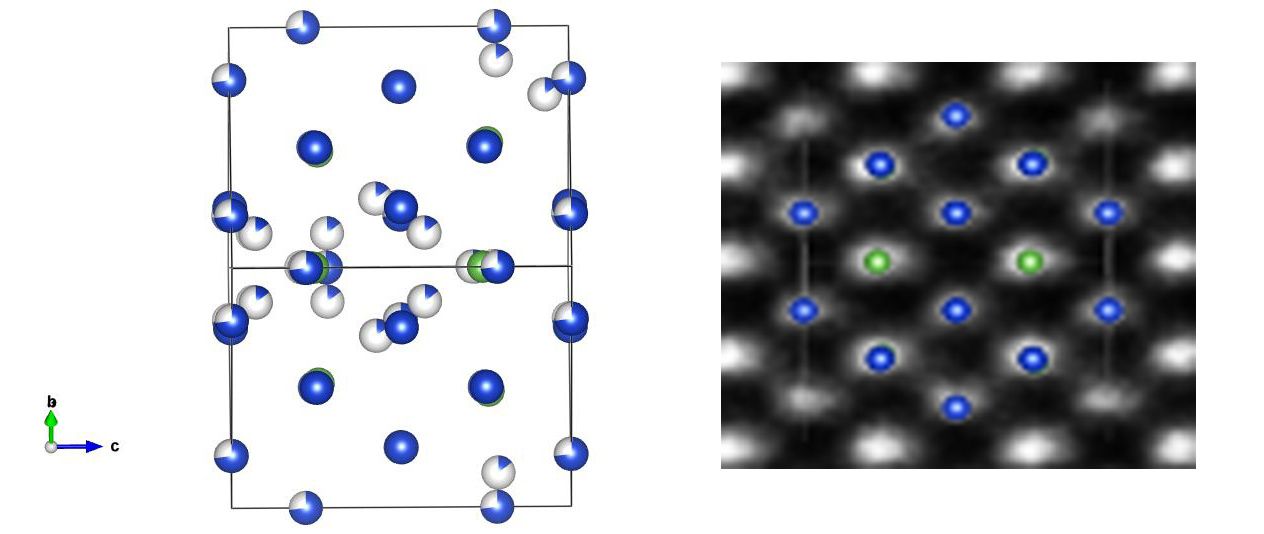
\includegraphics[width=0.48\textwidth]{mic_cu12as4s13_110}% Here is how to import EPS art
\caption{\label{fig:haadf_overlay} Left --- the tennantite crystal [110] zone  generated  by VESTA\cite{Momma2011}; rigth --- the HAADF image with the tennantite crystal [110] zone.}
\end{figure}


The full HAADF image with the tennantite crystal [110] zone and  transmission electron diffraction are shown in Fig.~\ref{fig:TEM}.

\begin{figure}
\centering
\subfigure{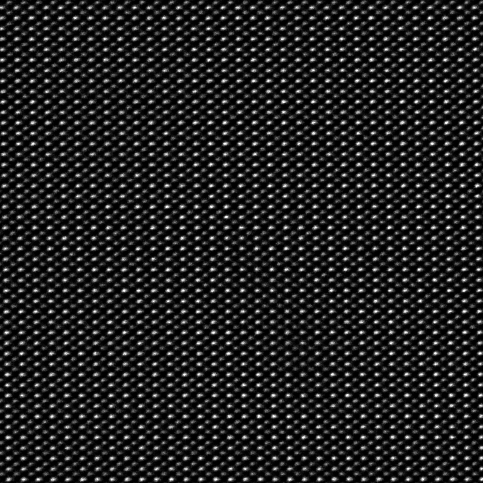
\includegraphics[width=0.2\textwidth]{mic_Figure_10}}
 \quad
\subfigure{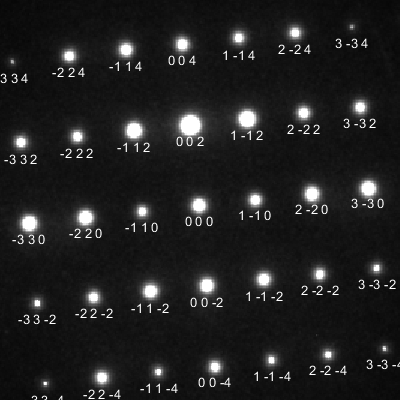
\includegraphics[width=0.2\textwidth]{difr01_el_mic_zone_110}}
\caption{\label{fig:TEM} Left --- the HAADF image with the tennantite crystal [110] zone , right --- transmission electron diffraction of the same zone. }
\end{figure}

\section{References}\label{sec:level1}
\bibliographystyle{elsarticle-num}
\bibliography{reff}

\end{document}
\endinput
%%
%% End of file `elsarticle-template-num.tex'.
